\documentclass[11pt, a4paper]{article}
\usepackage{pdfpages}
\usepackage{parallel}
\usepackage[T2A]{fontenc}
%\usepackage{ucs}
\usepackage[utf8]{inputenc}
\usepackage[english,russian]{babel}
\usepackage{hyperref}
\usepackage{rotating}
\usepackage[inner=2cm,top=1.8cm,outer=2cm,bottom=2.3cm,nohead]{geometry}
%\usepackage{listings}
\usepackage{graphicx}
\usepackage{wrapfig}
\usepackage{longtable}
\usepackage{indentfirst}
\usepackage{array}
\usepackage{tikzsymbols}
\usepackage{soul}
\usepackage[ruled,vlined]{algorithm2e}
\usepackage{qrcode}
\counterwithout{figure}{section} 

\usepackage{url}
\makeatletter
\g@addto@macro{\UrlBreaks}{\UrlOrds}
\makeatother

\newcolumntype{P}[1]{>{\raggedright\arraybackslash}p{#1}}
\frenchspacing
%\usepackage{fixltx2e} %text sub- and superscripts
\usepackage{icomma} % коскі ў матэматычным рэжыме
%\PreloadUnicodePage{4}

\newcommand{\longpage}{\enlargethispage{\baselineskip}}
\newcommand{\shortpage}{\enlargethispage{-\baselineskip}}

\def\switchlang#1{\expandafter\csname switchlang#1\endcsname}
\def\switchlangbe{
\let\saverefname=\refname%
\def\refname{Літаратура}%
\def\figurename{Іл.}%
}
\def\switchlangru{
\let\saverefname=\refname%
\let\savefigurename=\figurename%
\def\refname{Литература}%
\def\figurename{Рис.}%
}
\def\switchlangen{
\let\saverefname=\refname%
\def\refname{References}%
\def\figurename{Fig.}%
}

\hyphenation{admi-ni-stra-tive}
\hyphenation{ex-pe-ri-ence}
\hyphenation{fle-xi-bi-li-ty}
\hyphenation{Py-thon}
\hyphenation{ma-the-ma-ti-cal}
\hyphenation{re-ported}
\hyphenation{imp-le-menta-tions}
\hyphenation{pro-vides}
\hyphenation{en-gi-neering}
\hyphenation{com-pa-ti-bi-li-ty}
\hyphenation{im-pos-sible}
\hyphenation{desk-top}
\hyphenation{elec-tro-nic}
\hyphenation{com-pa-ny}
\hyphenation{de-ve-lop-ment}
\hyphenation{de-ve-loping}
\hyphenation{de-ve-lop}
\hyphenation{da-ta-ba-se}
\hyphenation{plat-forms}
\hyphenation{or-ga-ni-za-tion}
\hyphenation{pro-gramming}
\hyphenation{in-stru-ments}
\hyphenation{Li-nux}
\hyphenation{sour-ce}
\hyphenation{en-vi-ron-ment}
\hyphenation{Te-le-pathy}
\hyphenation{Li-nux-ov-ka}
\hyphenation{Open-BSD}
\hyphenation{Free-BSD}
\hyphenation{men-ti-on-ed}
\hyphenation{app-li-ca-tion}

\def\progref!#1!{\texttt{#1}}
\renewcommand{\arraystretch}{2} %Іначай формулы ў матрыцы зліпаюцца з лініямі
\usepackage{array}

\def\interview #1 (#2), #3, #4, #5\par{

\section[#1, #3, #4]{#1 -- #3, #4}
\def\qname{LVEE}
\def\aname{#1}
\def\q ##1\par{{\noindent \bf \qname: ##1 }\par}
\def\a{{\noindent \bf \aname: } \def\qname{L}\def\aname{#2}}
}

\def\interview* #1 (#2), #3, #4, #5\par{

\section*{#1\\{\small\rm #3, #4. #5}}
\ifx\ParallelWhichBox\undefined%
    \addcontentsline{toc}{section}{#1, #3, #4}%
\else%
\ifnum\ParallelWhichBox=0%
    \addcontentsline{toc}{section}{#1, #3, #4}%
\fi\fi%

\def\qname{LVEE}
\def\aname{#1}
\def\q ##1\par{{\noindent \bf \qname: ##1 }\par}
\def\a{{\noindent \bf \aname: } \def\qname{L}\def\aname{#2}}
}

\newcommand{\interviewfooter}[1]{
\vskip 1em
\noindent \textit{#1}
}

\AtEndDocument{\vfill\centering \qrcode{https://github.com/fiowro/mouses/blob/main/\jobname.pdf}}

\switchlang{en}
\begin{document}

\title{1985 "--- Microsoft Gray-eyed Mouse}
\date{}
\maketitle
\selectlanguage{english}

This mouse, which went on sale in 1985, became a second generation of Microsoft mice. The company simply called its early models ``Microsoft mouse'', sometimes also specifying the method of connection to the computer. Therefore, the official name of this one, ``Microsoft Serial Mouse'', was rather confusing, and the mouse became known among users as the ``Microsoft Gray-Eyed Mouse'' (to differentiate it from the first generation mice with a pair of green buttons known under the ``Green-Eyed Mouse'' nickname). Also sometimes this mouse is referred to as ``Microsoft Mouse 5.0'' \cite{mouses}, apparently due to the variants of the first generation mice with different interfaces.
The real manufacturer of the mouse, as in the case of the first generation, was the Japanese company Alps.

\begin{figure}[h]
   \centering
    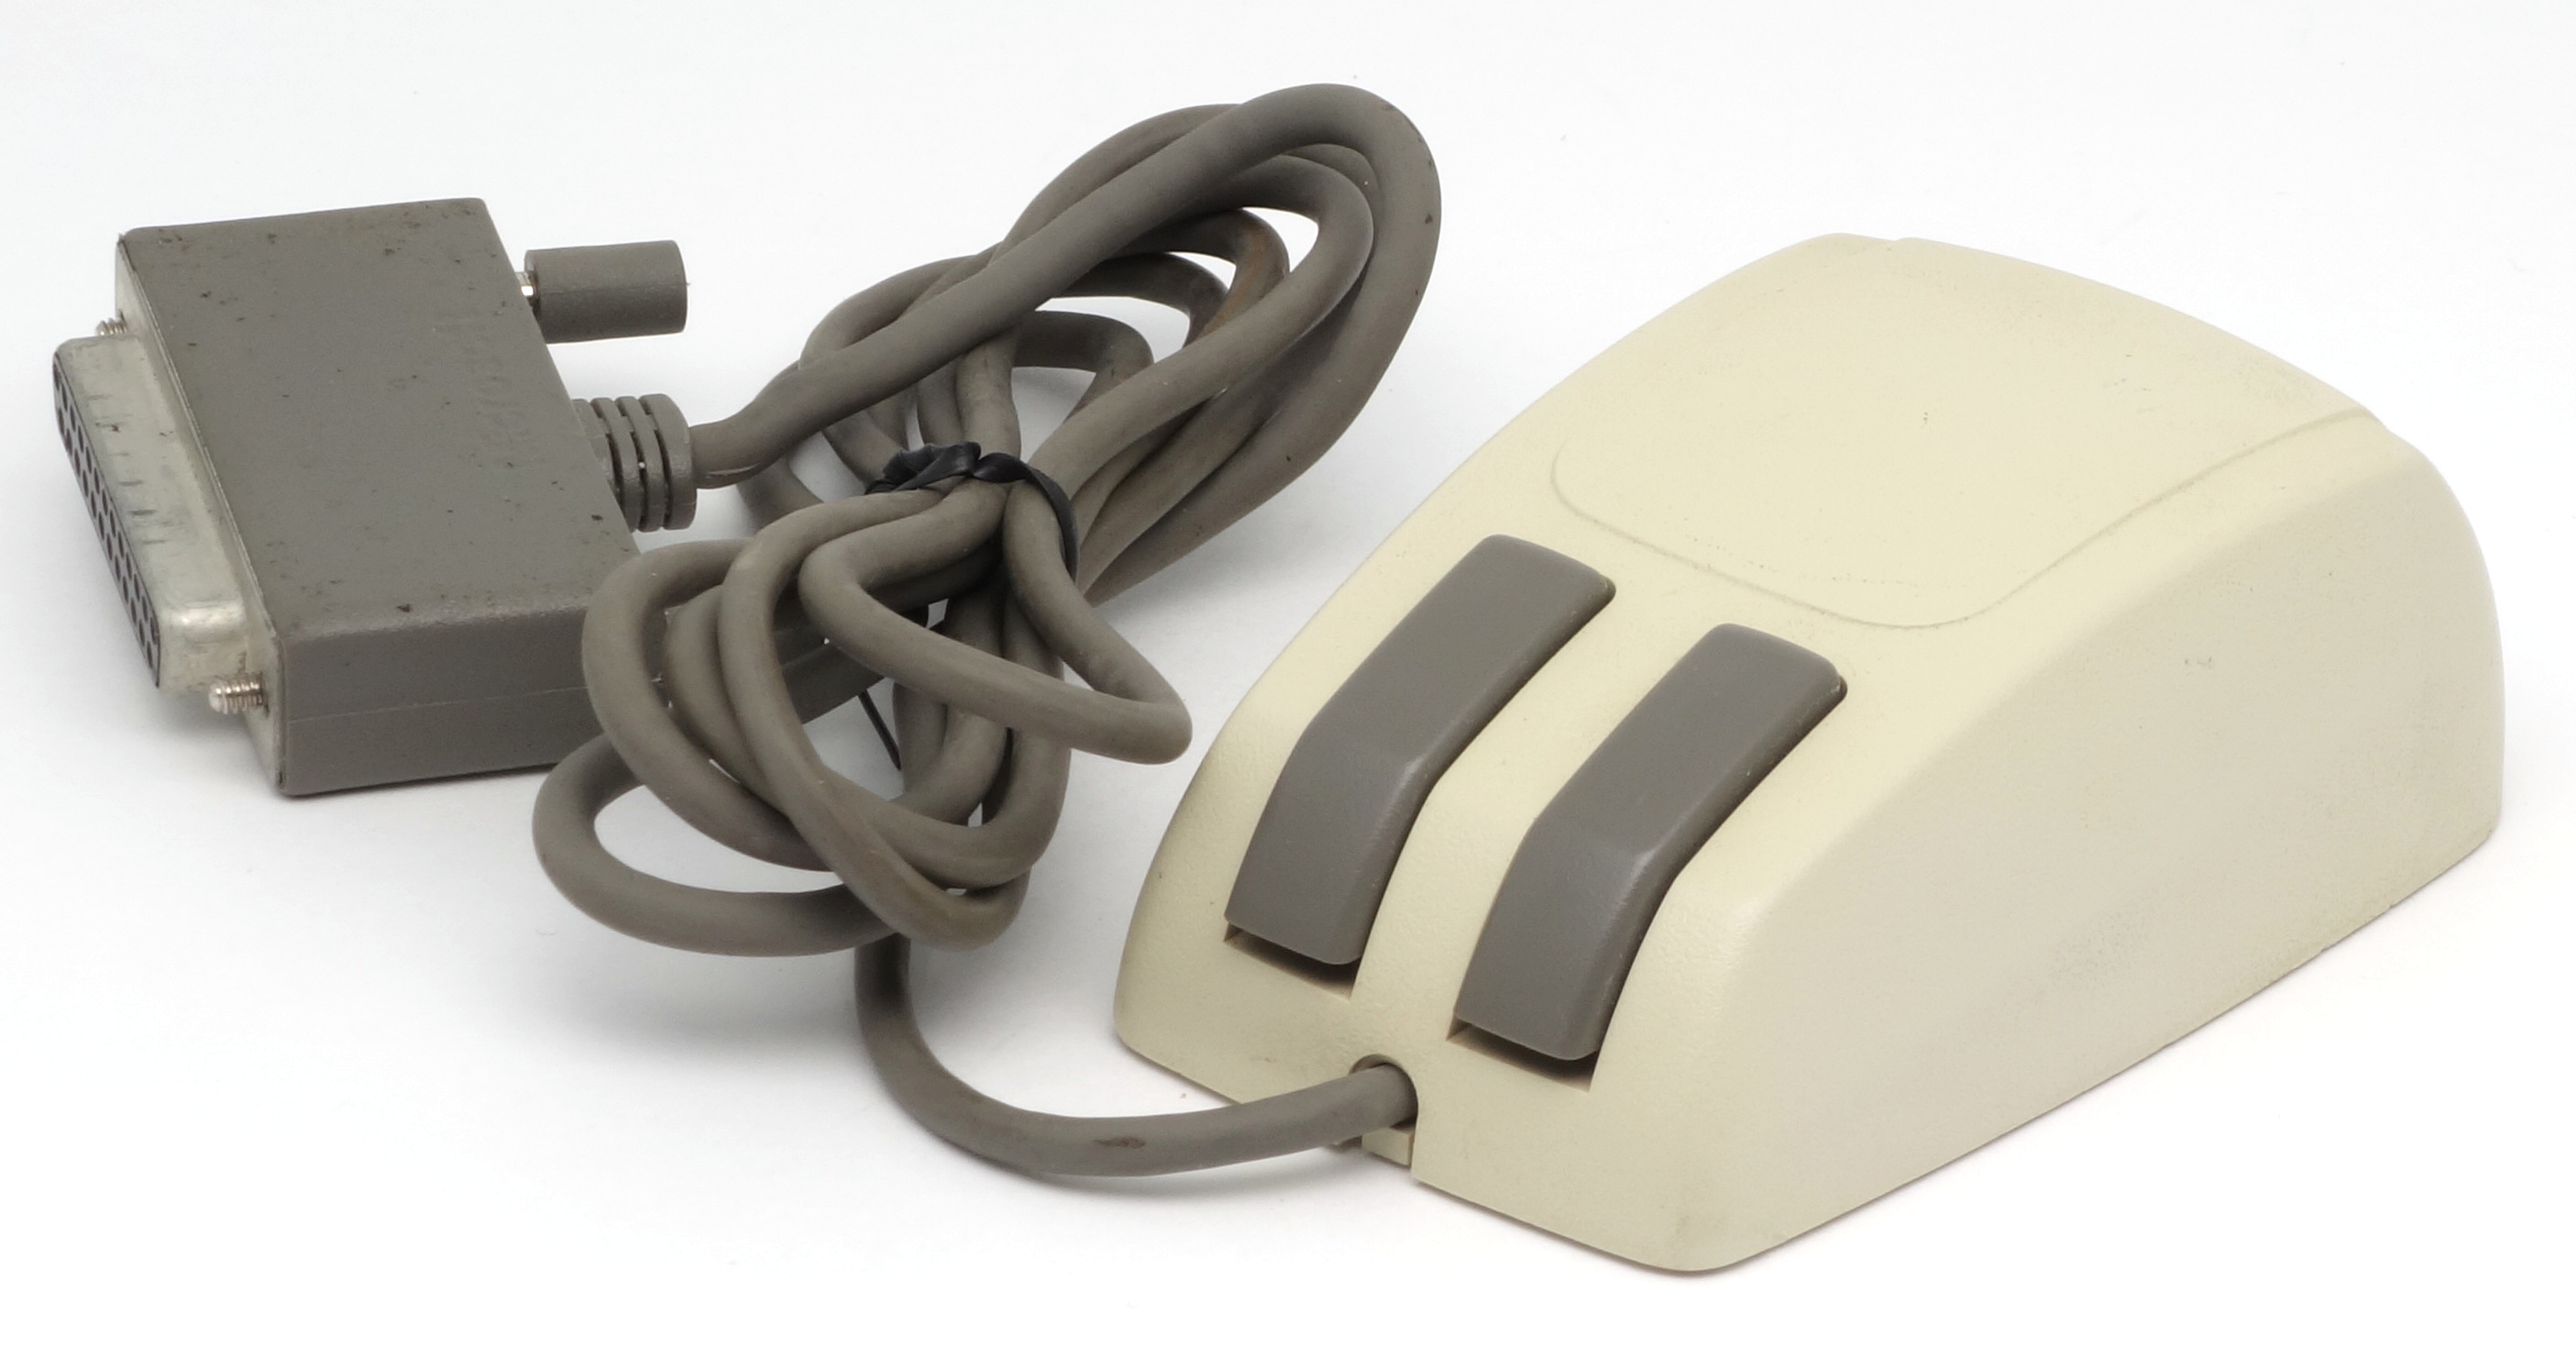
\includegraphics[scale=0.55]{1985_microsoft_gray_eyed_mouse/pic_30.jpg}
    \caption{Microsoft Gray-eyed Mouse}
    \label{fig:MicrosoftGrayEyedPic}
\end{figure}

The second generation received several significant improvements in both design and ergonomics. The body material is classic beige plastic, and the body itself has become more convex. Two contrasting gray buttons are still located on the sloping front edge, but also extend onto the top of the body (fig. \ref{fig:MicrosoftGrayEyedPic}). Just for the note, there are also examples of the ``Gray-eyed'' Microsoft mouse with red buttons.

\begin{figure}[h]
    \centering
    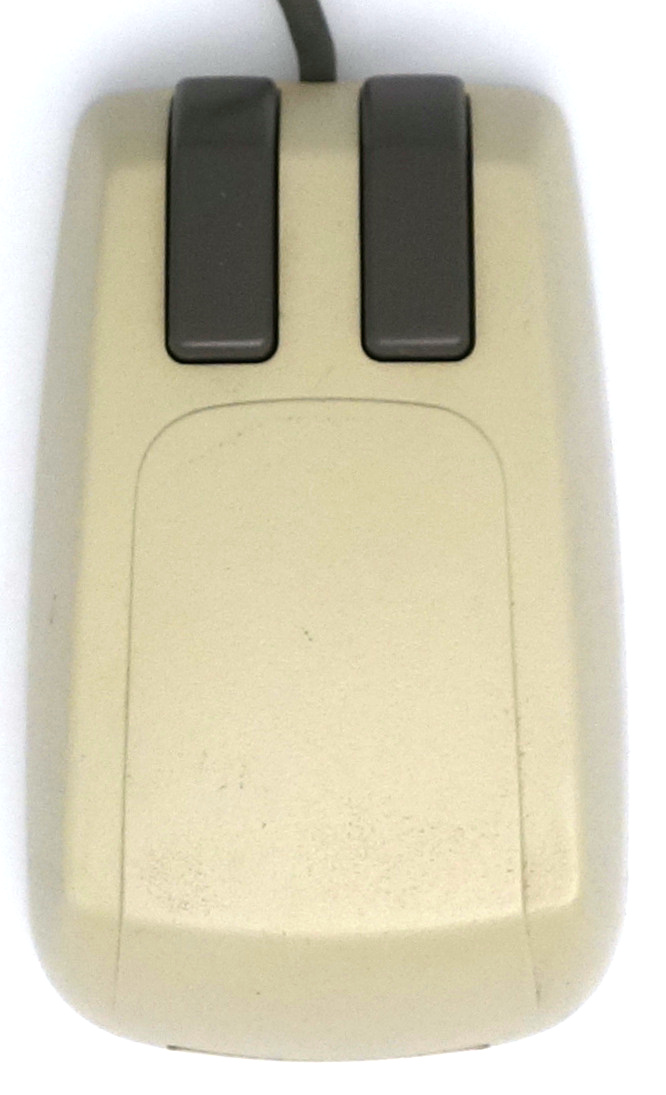
\includegraphics[scale=0.6]{1985_microsoft_gray_eyed_mouse/top_30.jpg}
    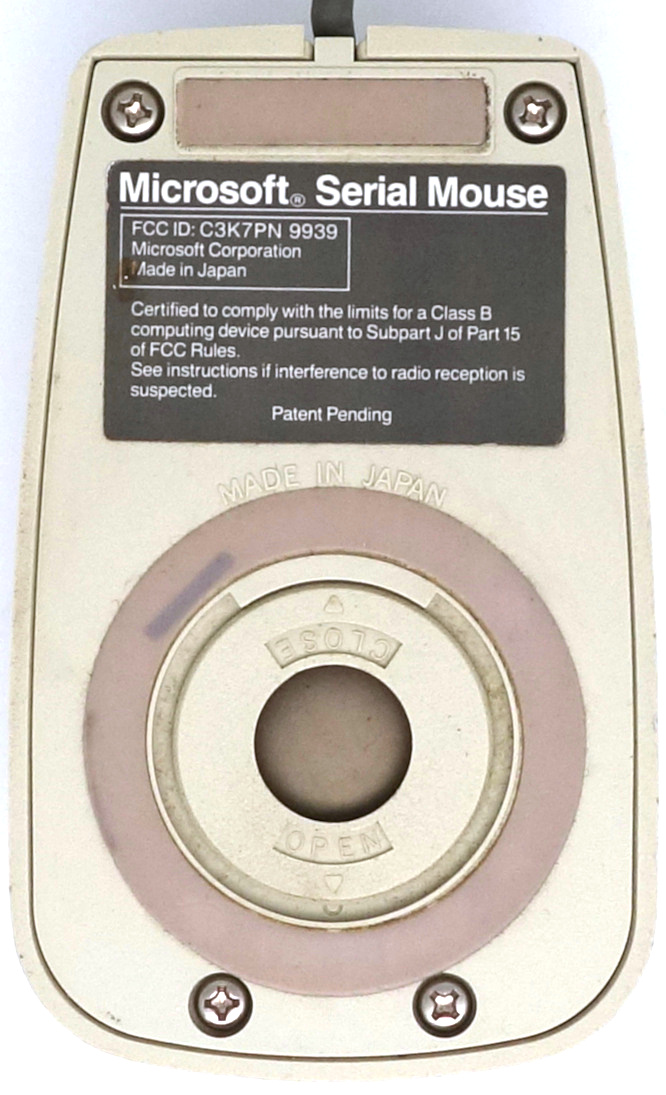
\includegraphics[scale=0.6]{1985_microsoft_gray_eyed_mouse/bottom_30.jpg}
    \caption{Microsoft Gray-eyed Mouse, top and bottom views}
    \label{fig:MicrosoftGrayEyedTopAndBottom}
\end{figure}

The bottom contains a rubber-coated ball and a locking ring that can be pushed to the side to remove the ball for cleaning the mouse (fig. \ref{fig:MicrosoftGrayEyedTopAndBottom}). Around the locking ring there is a contrasting ring-shaped pad made of low-friction material, which is a hallmark of many mice of the 80s designed in Japan. The rubber-coated ball was an important advantage over the green-eyed mouse's regular steel ball: it both reduced ball slippage and ensured quiet operation of the mouse on hard surfaces.

\begin{figure}[h]
    \centering
    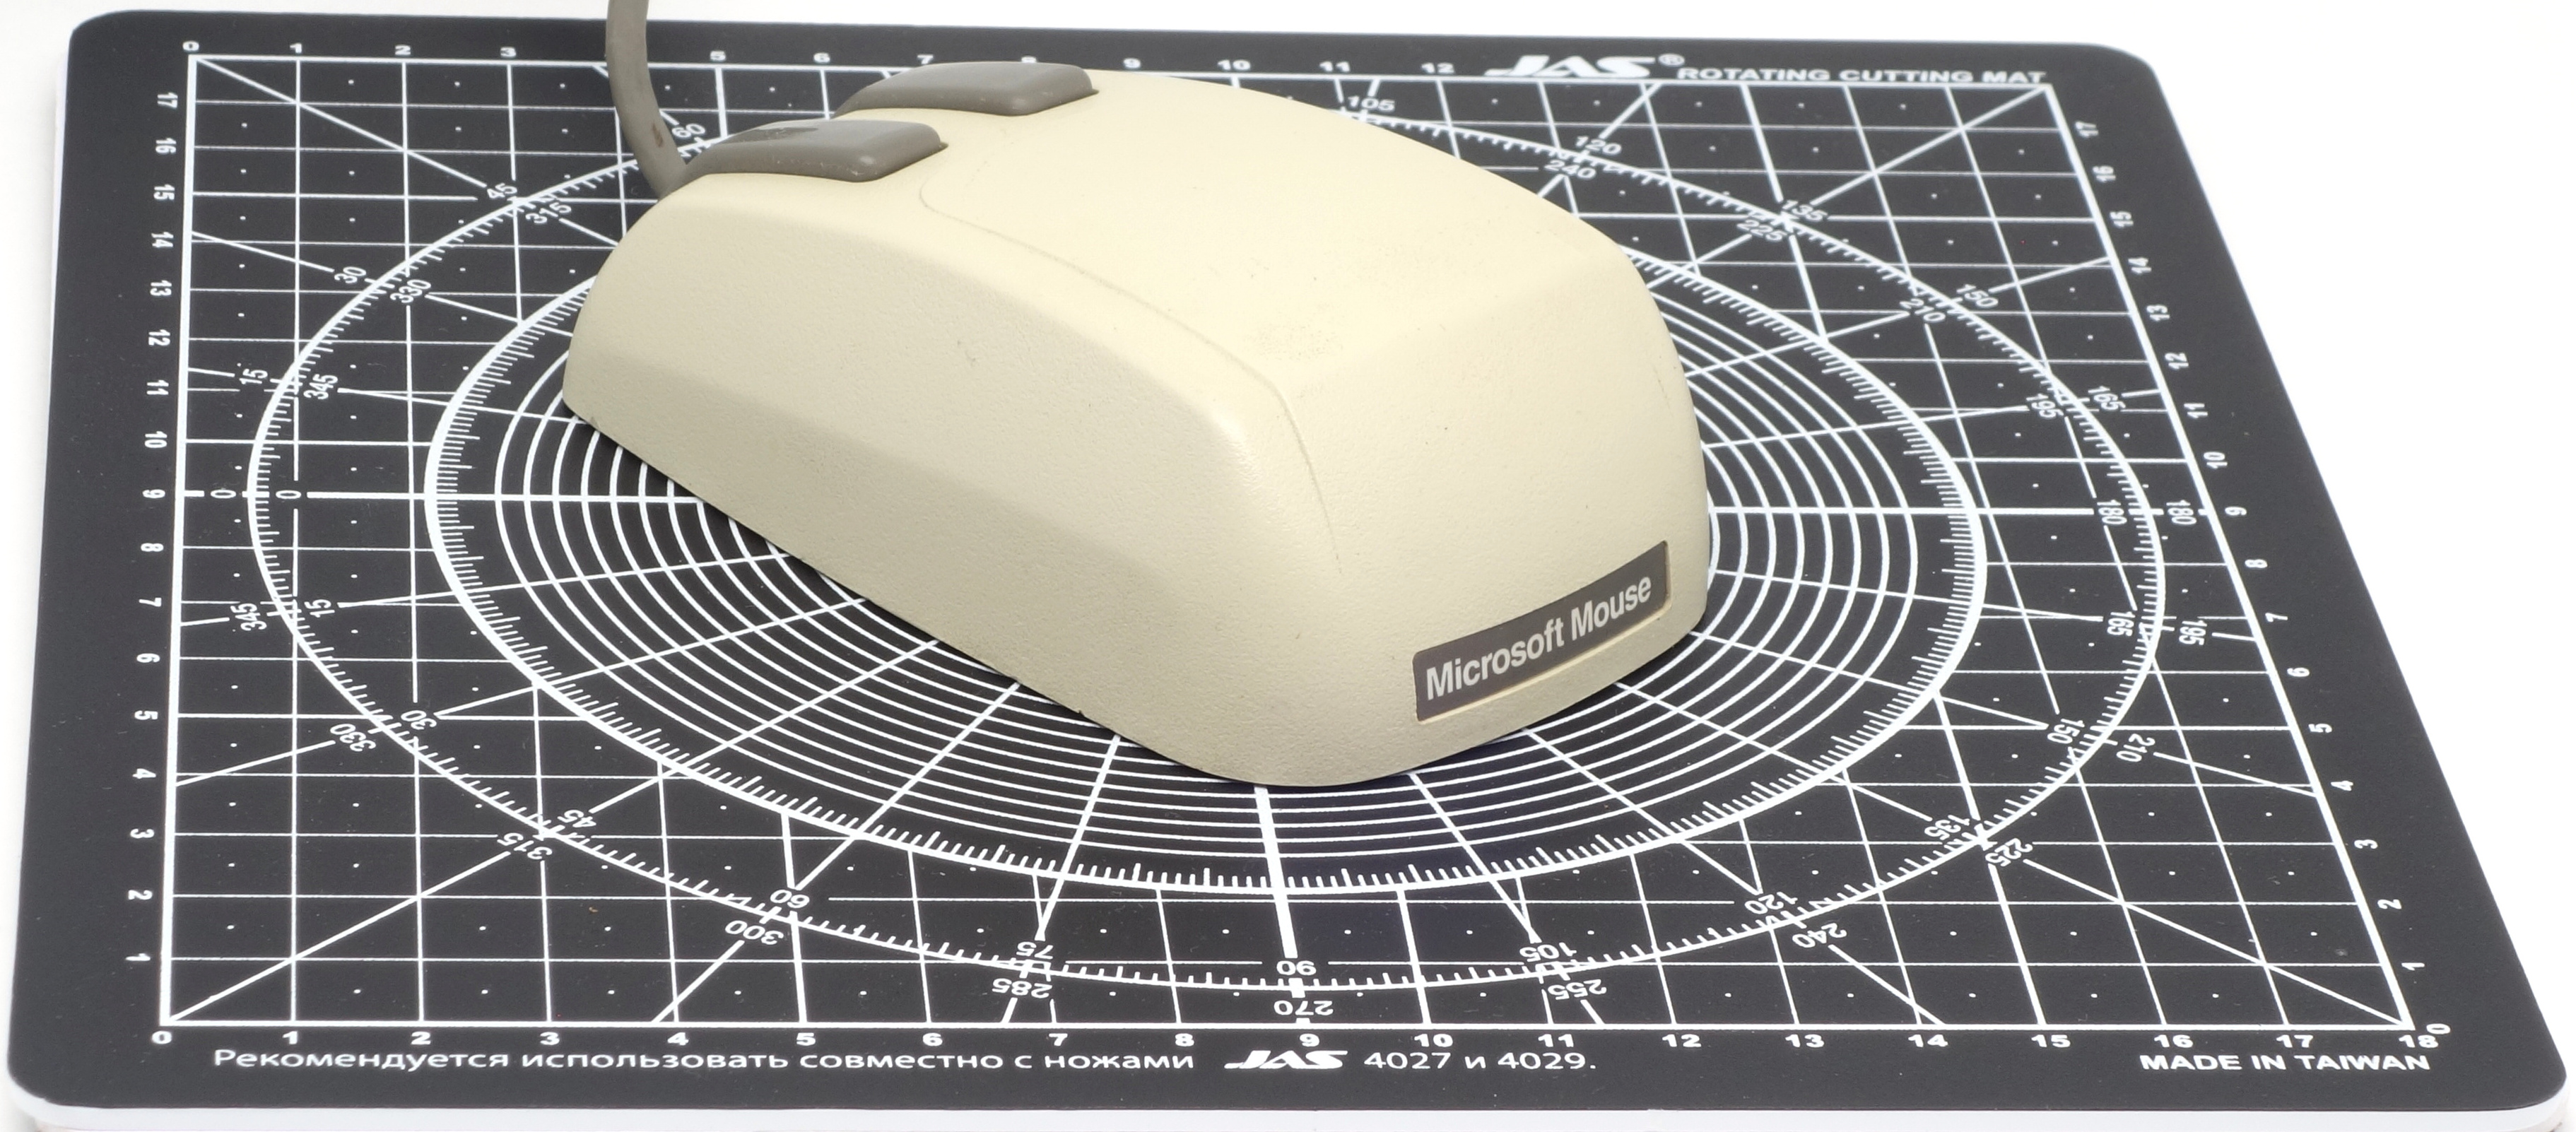
\includegraphics[scale=0.5]{1985_microsoft_gray_eyed_mouse/size_30.jpg}
    \caption{Microsoft Gray-eyed Mouse on a graduated pad with a grid step of 1~cm}
    \label{fig:MicrosoftGrayEyedSize}
\end{figure}

The size of the mouse is typical for the 80s (Fig. \ref{fig:MicrosoftGrayEyedSize}) and is determined by the dimensions of the used ALPS unit. In promotional materials, Microsoft emphasizes that ``the wrap-around command buttons designed to fit naturally in the palm of any size hand'' \cite{mouses}. Some of the criticism of the ergonomics of the first generation of mice concerned the ability to move the mouse by pressing the buttons on the front wall of the case, and this double position of the buttons apparently solved this problem, allowing those who were more comfortable to press them from above (fig. \ref{fig: MicrosoftGrayEyedHand}). Following Microsoft, this angular button shape appeared in several more mice. The most similarities, down to the similar body shape, are demonstrated by the ProCorp Serial Mouse from 1988 and the Vatek Color Mouse from 1989.

\begin{figure}[h]
    \centering
    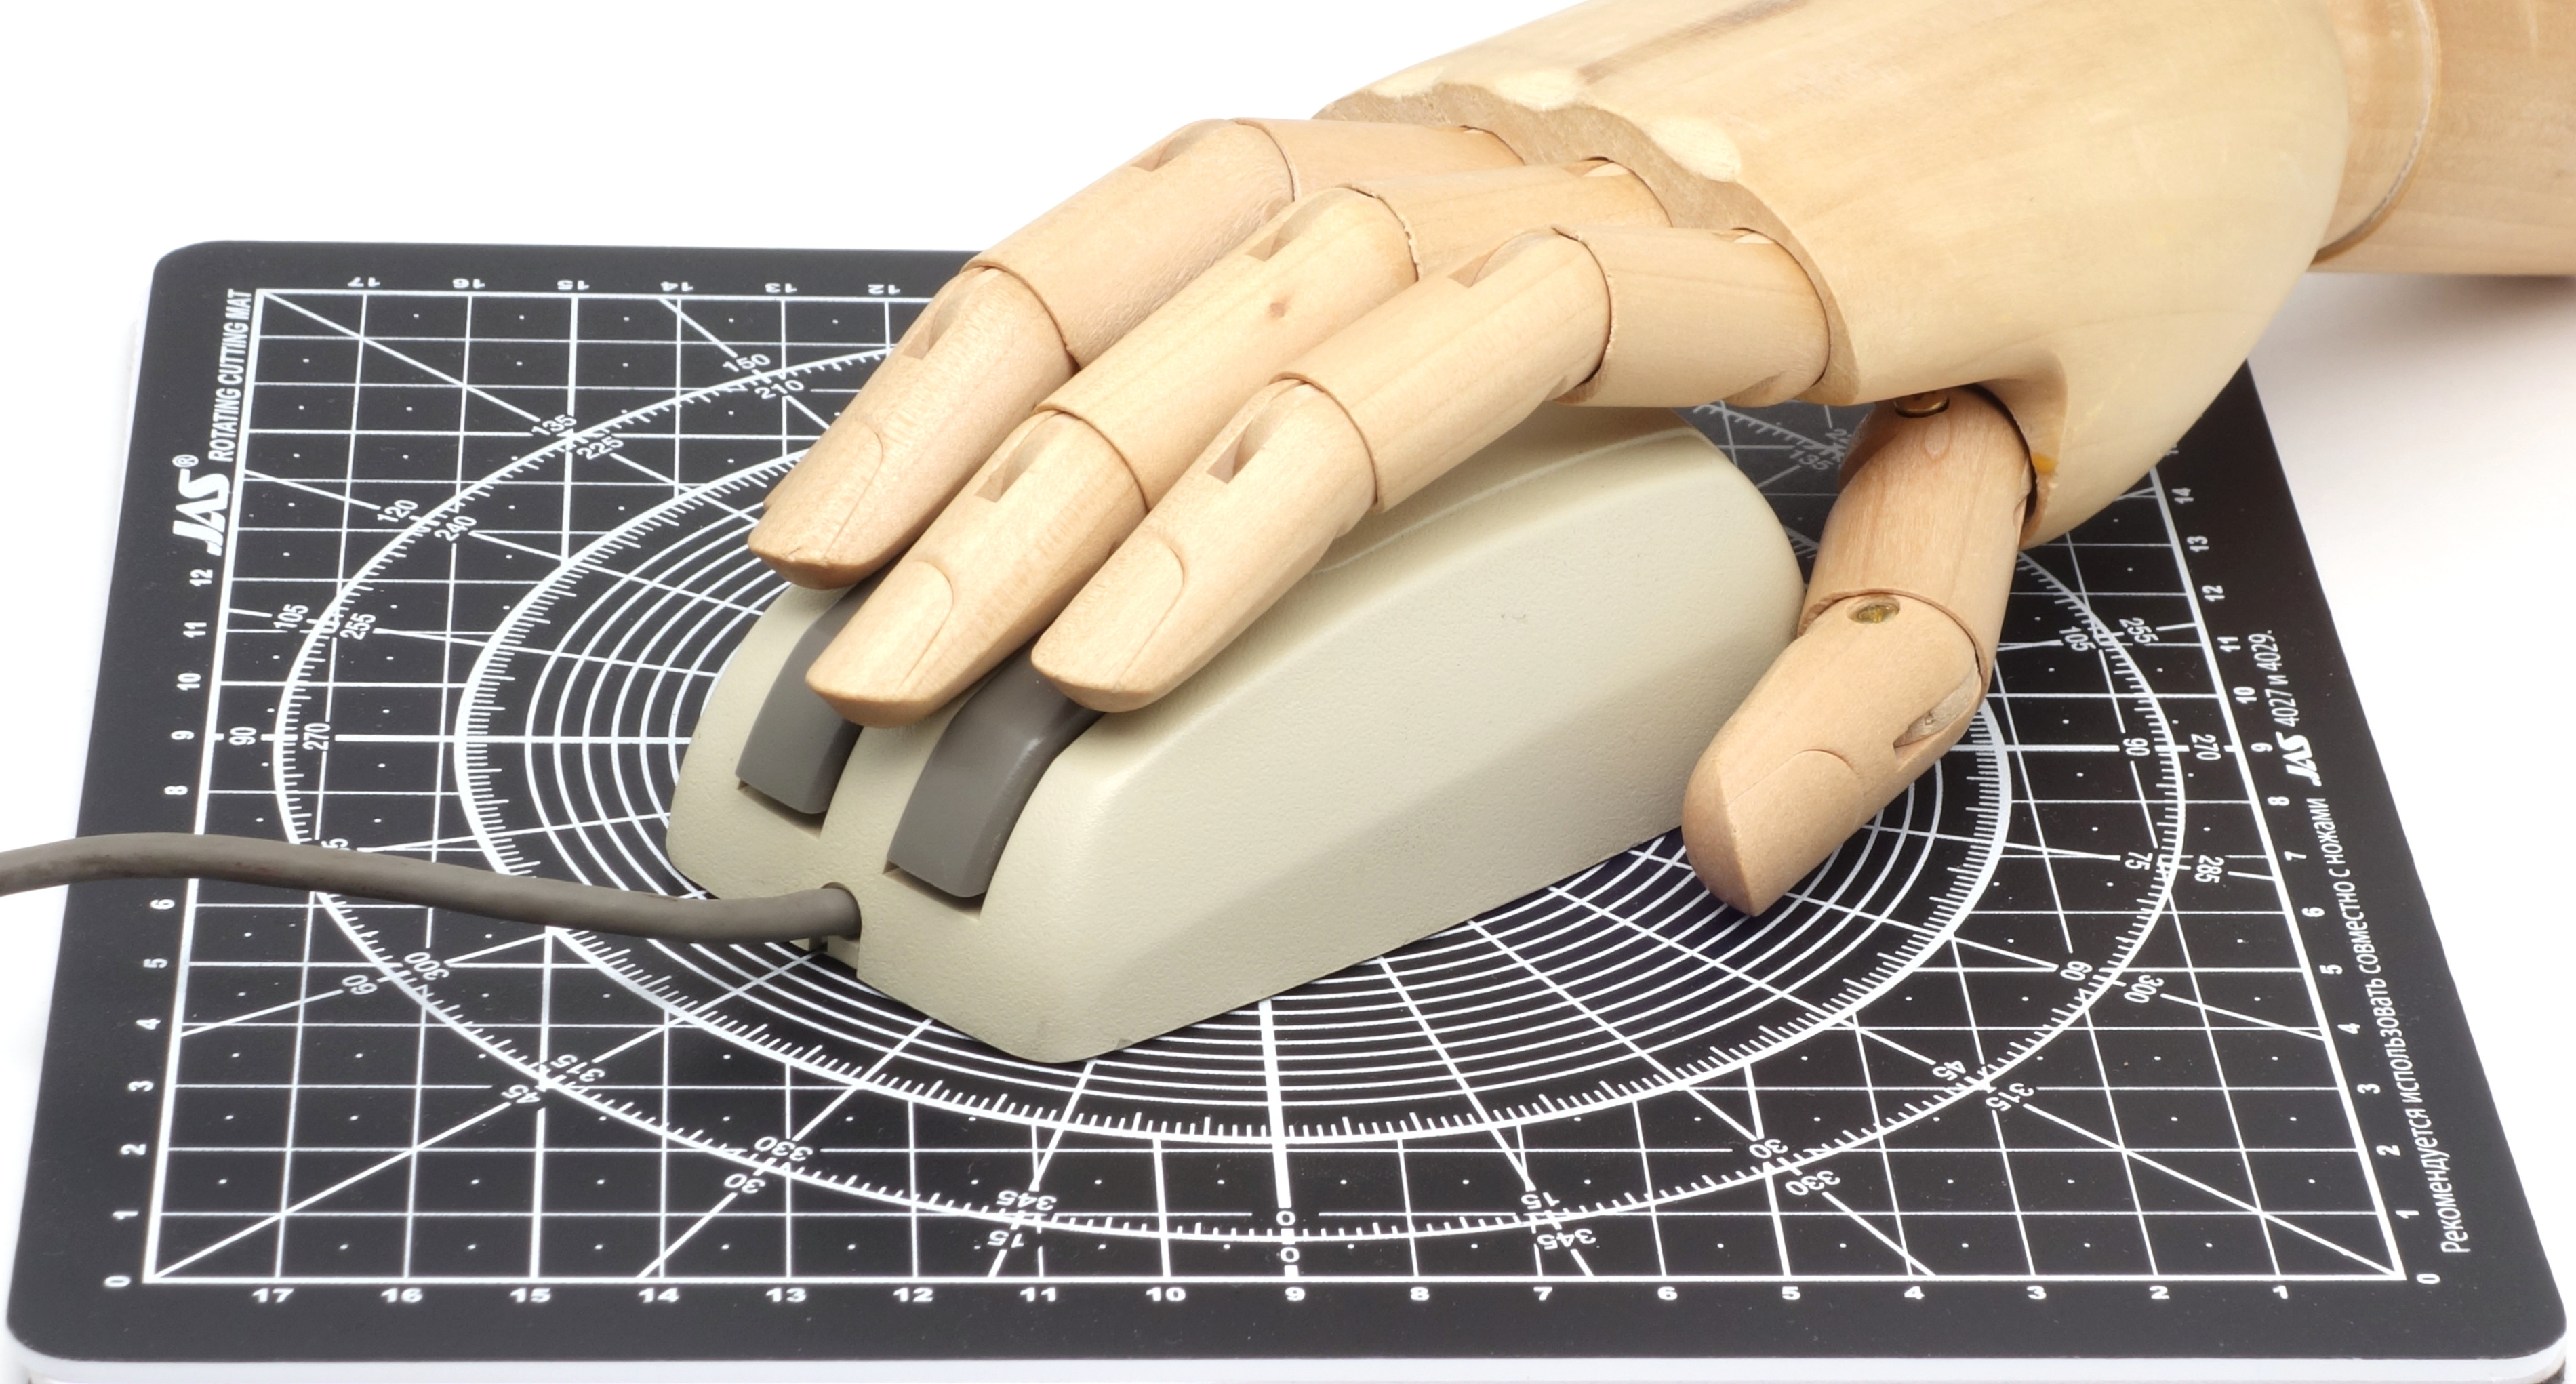
\includegraphics[scale=0.5]{1985_microsoft_gray_eyed_mouse/hand_30.jpg}
    \caption{Microsoft Gray-eyed Mouse with a human hand model}
    \label{fig:MicrosoftGrayEyedHand}
\end{figure}

The Microsoft promo also noted ``twice the resolution of most other mice—200 points per inch'' (``most other mice'' in this case meant just Microsoft's first generation mice).

This mouse sample has a serial connection interface. In addition, this model was produced as a quadrature mouse in two versions \cite{guide}: with a bus interface (complete with a special adapter board) and with the InPort interface (Microsoft’s attempt to standardize the interface for connecting quadrature mice, the corresponding adapters and converters for them). It is worth noting that the first two generations of Microsoft mice with a serial interface have the same FCC ID code, so in fig. \ref{fig:MicrosoftGrayEyedTopAndBottom} you can see the FCC ID of the ``green-eyed'' mouse, registered in 1983 \cite{zero}. 

\begin{figure}[h]
    \centering
    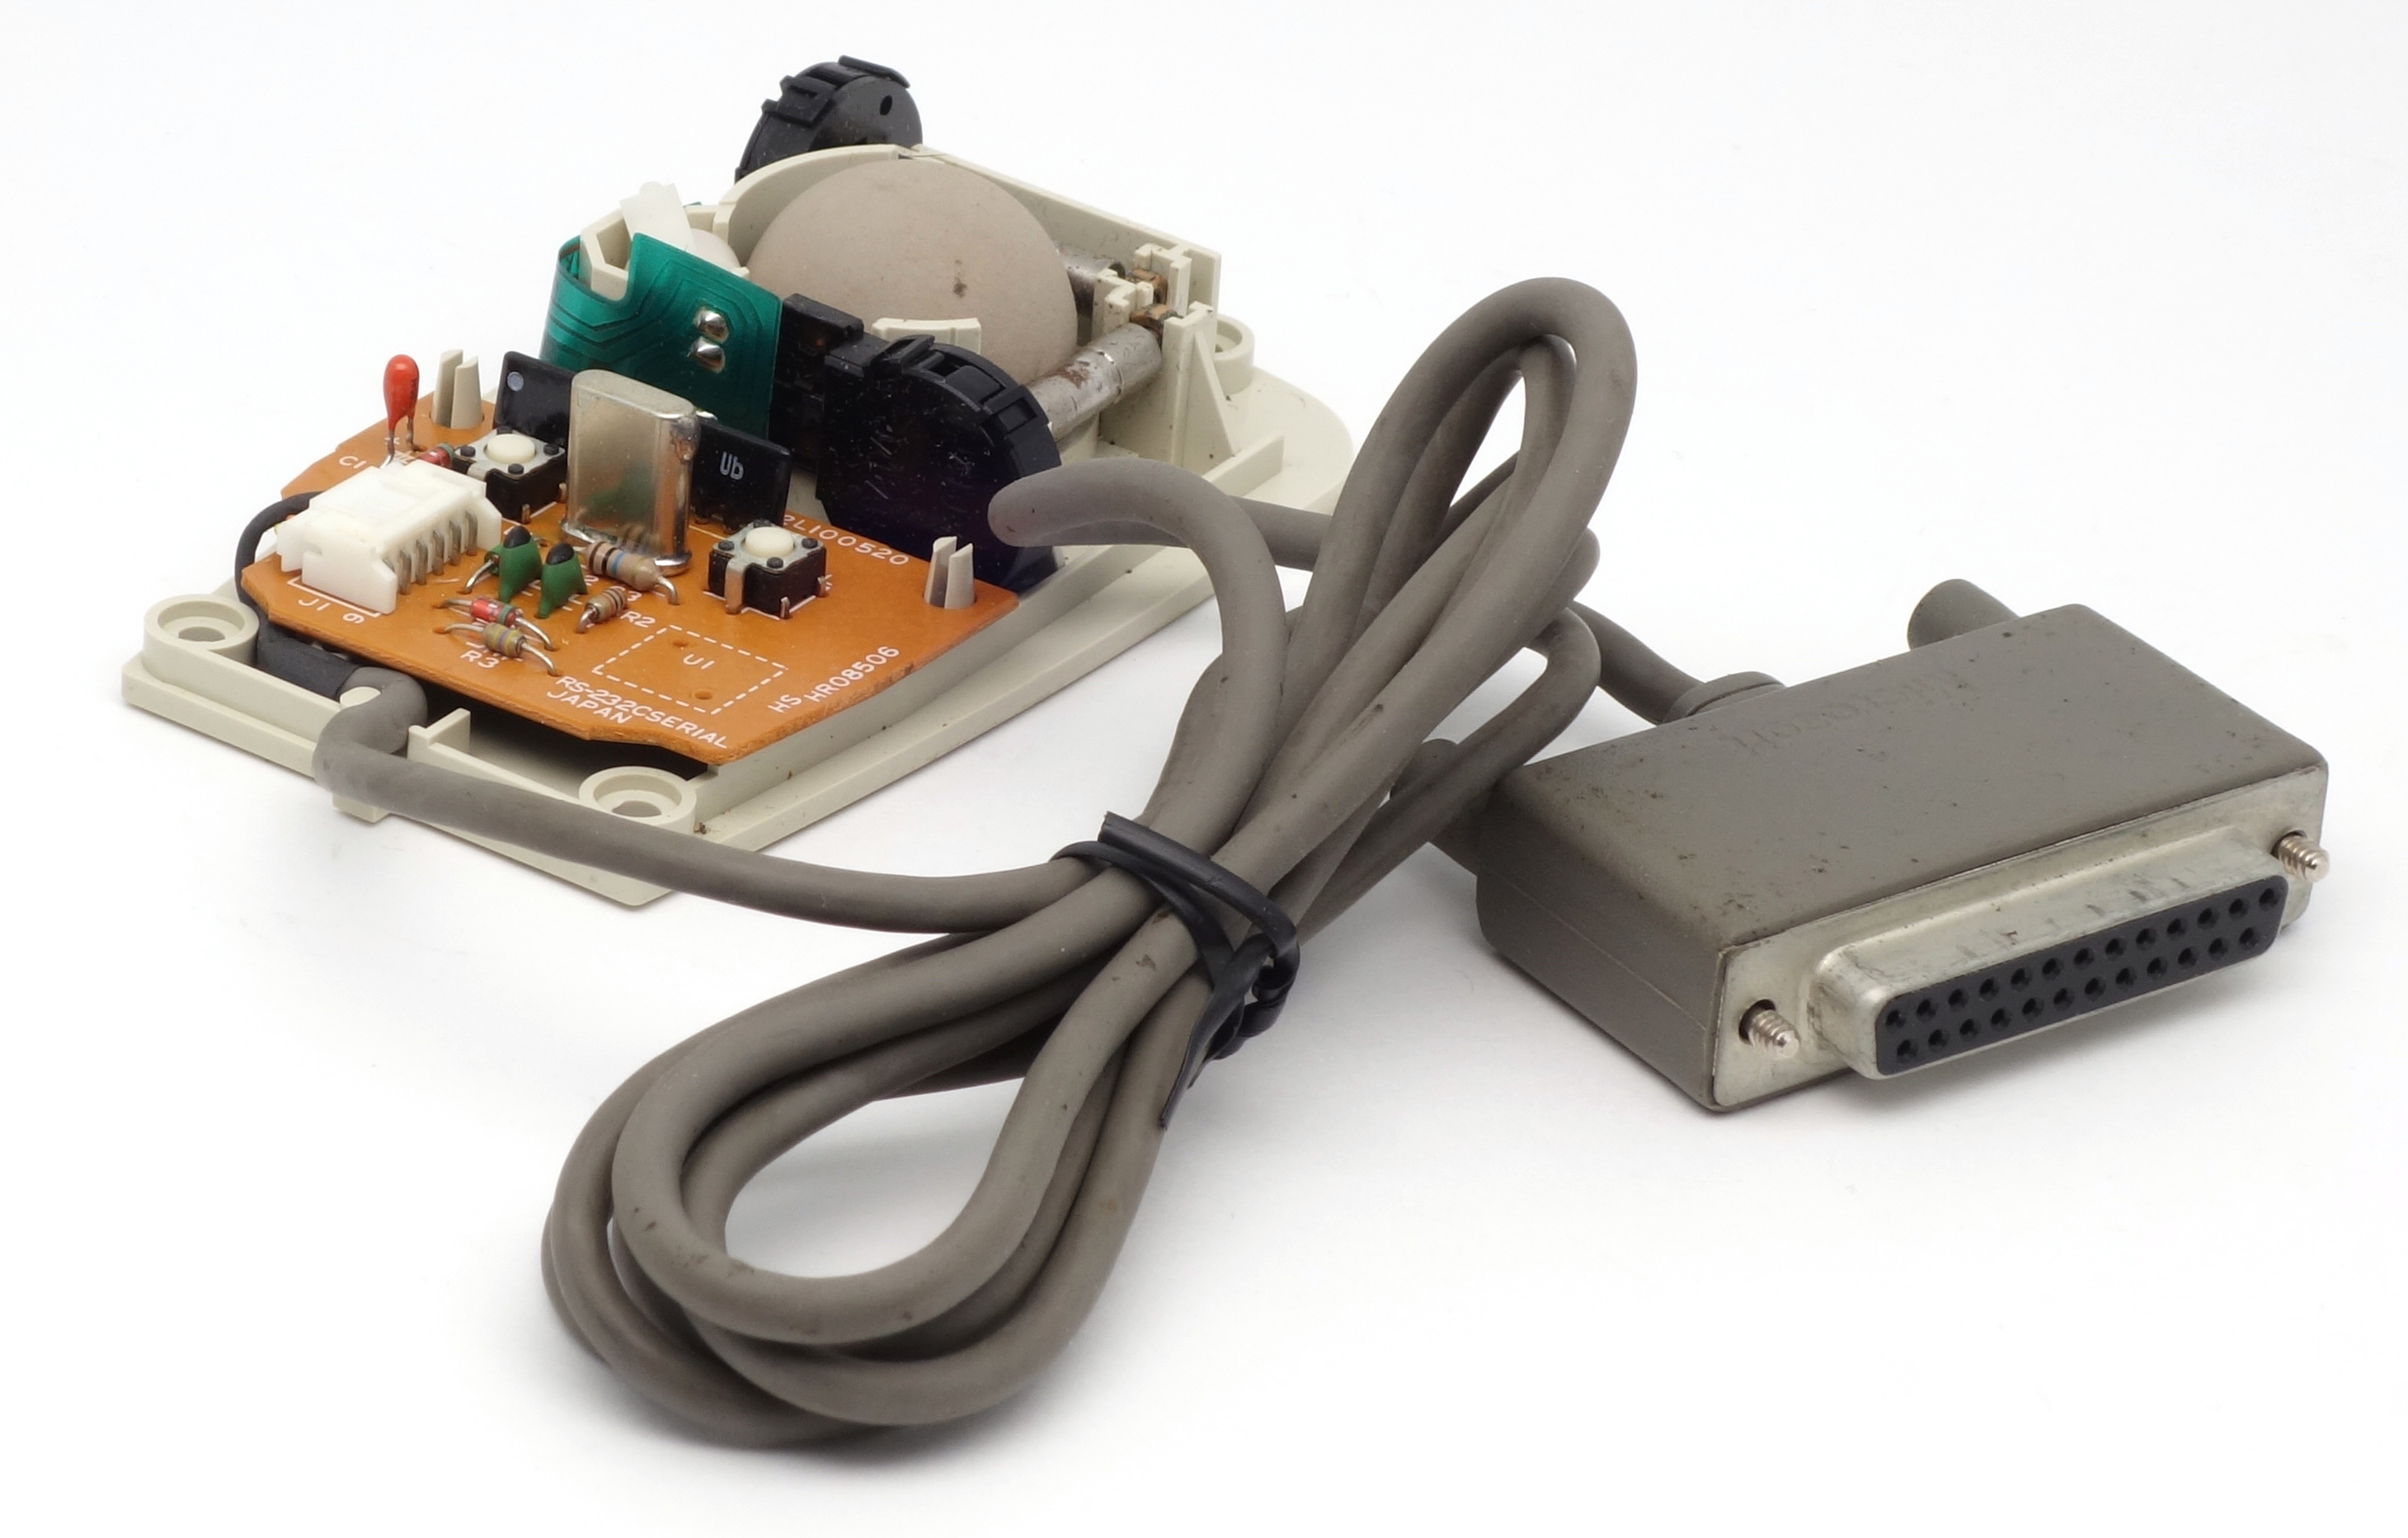
\includegraphics[scale=0.5]{1985_microsoft_gray_eyed_mouse/inside_30.jpg}
    \caption{Microsoft Gray-eyed Mouse disassembled}
    \label{fig:MicrosoftGrayEyedInside}
\end{figure}

The internal structure of the mouse can be seen in fig. \ref{fig:MicrosoftGrayEyedInside}. Apparently, the real manufacturer of the mouse was the Japanese company Alps, which often acted as a contractor in the development of mice for other companies (examples of such companies are IBM, Sharp, NeXT,  Siemens, Intergraph). Alps usually designed mouse with a unique body shape and buttons layout for each customer, but used the same implementation for several devices. In particular, this mouse has identical parts (the lower part of the body, massive metal rollers with bearings, a movement registration unit based on closed mechanical encoders connected to a double-sided printed circuit board by a T-type ribbon cable) with the original mouse of NeXT computers produced since 1988, with the Panasonic FS-JM650 mouse sold in 1986, and with IBM PS/2 Mouse, produced in 1987.

\begin{thebibliography}{9}
\bibitem{mouses} Microsoft Gray-eyed Mouse \url{https://web.archive.org/web/20210417233303/http://oldmouse.com/mouse/microsoft/grayeyed.shtml}
\bibitem{guide} Microsoft Mouse User Guide. Microsoft, 1986. \url{https://minuszerodegrees.net/manuals/Microsoft/Microsoft%20Mouse%20-%20User's%20Guide%20-%201986.pdf}
\bibitem{zero} Microsoft Mouse. Minus zero degrees \url{https://www.minuszerodegrees.net/msmouse/Microsoft%20mouse.htm}
\end{thebibliography}
\end{document}
